%----------------------------------------------------------------------------
\chapter*{\bevezeto}\addcontentsline{toc}{chapter}{\bevezeto}
%----------------------------------------------------------------------------

Napjainkban a teljesítményelektornikai eszköz egyre inkább hangsúlyosabb szereplőivé válnak életünknek és az iparnak. A modern hajtástechnikai eszközök mind a hatékonyságot, mind a környezettudatos, fenntartható energiagazdálkosát is biztosítják. Az elektromos közlekedés nagyon jó példája ennek a folymatnak. Néhány éve még csak cikkekben olvashattunk ilyen járművekről, ma már teljesen természetes szereplői a forgalomnak, valamint a jogalkotás is követi már a folyamatot, megjelent a köztudatban is a "zöld rendszám" fogalma. 

Egy ilyen jármű esetében rögtön kettő felhasználási lehetőséget is találunk. Az első, amikor az autónkat tölteni kívánjuk. Egy ilyen töltő esetében fontos elvárás, hogy minél nagyobb teljesítményű legyen, hiszen minél rövidebb idő alatt fel akarjuk tölteni az autót. Fontos továbbá, hogy minél kisebb is legyen, hiszen nem csak otthon akarunk tölteni, ezért minél kisebbnek és könnyebbnek is kell lennie, hogy az autóba beépíthetővé váljon anélkül, hogy sok hasznos teret elvenne, vagy jelentősen növelné az autó tömegét. \Aref{fig:brusa} ánrán látható a svájci BRUSA cég On-board\footnote{fedélzeti} tötője.

\begin{figure}[!ht]
	\centering
	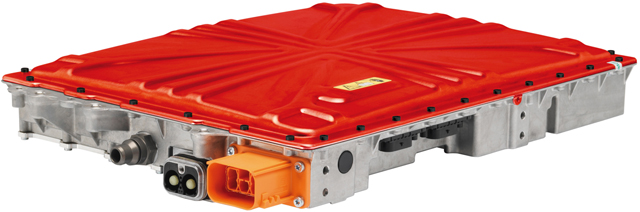
\includegraphics[width = \textwidth]{figures/brusa_charger.jpg}
	\caption{A svájci BRUSA cég "On-board" töltője} 
	\label{fig:brusa}
\end{figure}

\paragraph
A következő probléma az akkumulátorban tárolt energia felhasználása a jármű hajtására. Ehhez nyilvánvalóan szükség van egy motorra, amely többnyire háromfázisú szinkrongép. A fenti elvárások most is adottak, hiszen a ezt az eszközt is folyamatosan magunkkal kell vinni, illetve itt még a kétirányú eneriaáramlást is illik biztosítani, hiszen a regeneratív fékezés ma már jogosan elvárt funkció. 

Fenti -- és még sok más egyéb -- húzóágazatok miatt egyre inkább gyorsul a teljesítmény-átalakító eszközök fejlődése, ennélfogva, hogy piacképes terméket lehessen előállítani a fejlesztési időknek is egyre gyorsulnia kell. Ezt támogató eszköz a \emph{Hardware in the Loop} szimuláció. 


\begin{figure}[!ht]
	\centering
	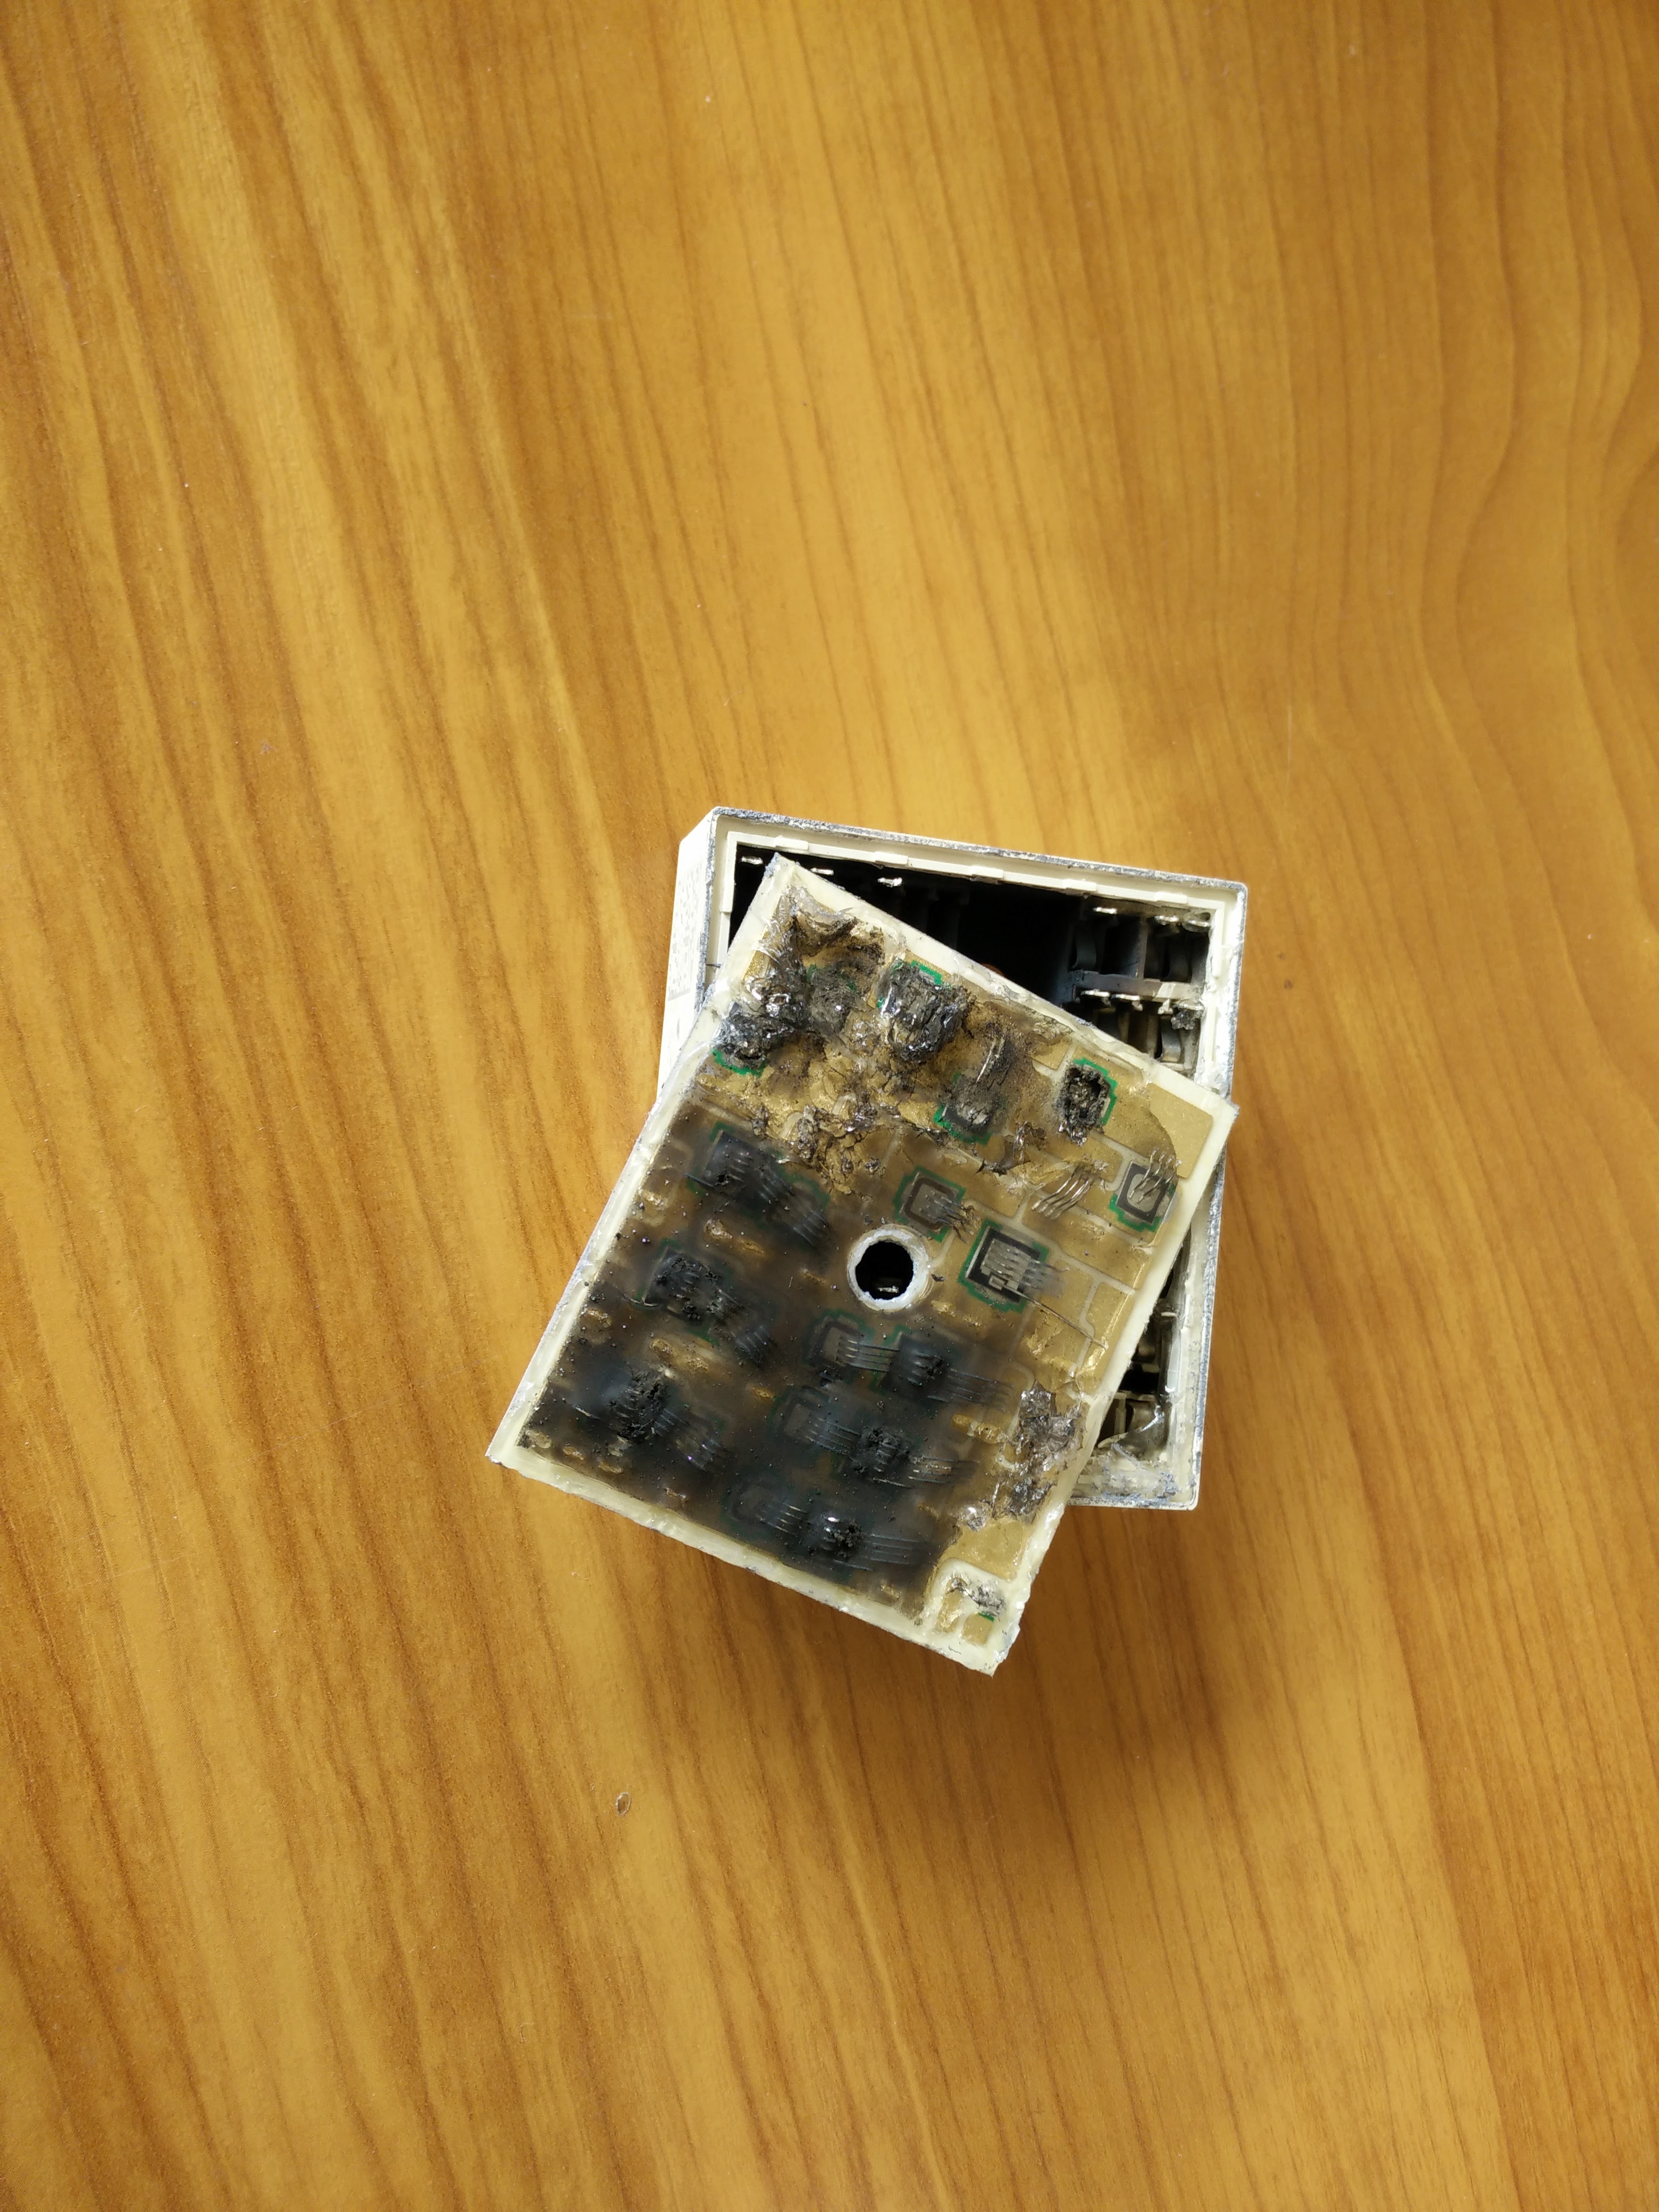
\includegraphics[scale = 0.05]{figures/IMG_20160415_134241.jpg}
	\caption{Felrobbant IGBT modul} 
	\label{fig:blown}
\end{figure}